\section{DIAGNÓSTICO DE LA TI SITUACIÓN ACTUAL}
\subsection{Capacidades del área de TI}
    Basándonos en la información disponible, podemos inferir que Alicorp ha desarrollado un sólido ecosistema tecnológico, destacando en las siguientes áreas: 

        \paragraph*{Gestión de la Cadena de Suministro} 
        Alicorp ha invertido significativamente en la implementación de sistemas ERP (Enterprise Resource Planning) que integran y automatizan diversas funciones de la cadena de suministro, desde la planificación de la producción hasta la gestión de inventario y la distribución. Estos sistemas permiten a la empresa: 
        Optimizar la planificación de la producción: Al contar con datos precisos sobre la demanda y el inventario, Alicorp puede ajustar su producción de manera más eficiente, evitando sobrestocks y faltantes. 
        Mejorar la gestión de inventario: Los sistemas ERP permiten un seguimiento en tiempo real del inventario, lo que reduce los costos asociados a la sobreproducción o a la falta de stock. 
        Optimizar las rutas de distribución: Mediante el uso de herramientas de análisis de datos y algoritmos de optimización, Alicorp puede planificar las rutas de distribución de manera más eficiente, reduciendo costos y tiempos de entrega. 
        Aumentar la visibilidad de la cadena de suministro: El IoT (Internet de las Cosas) juega un papel fundamental al permitir el seguimiento en tiempo real de los productos a lo largo de toda la cadena de suministro, desde la materia prima hasta el consumidor final. Esto facilita la identificación de posibles problemas y la toma de decisiones más ágiles. 

        \paragraph*{Producción}
        La aplicación de las TICs en los procesos productivos de Alicorp ha permitido mejorar significativamente la eficiencia y la calidad. Algunos ejemplos son: 
        Automatización de procesos: La implementación de robots y sistemas automatizados en las líneas de producción ha reducido los errores humanos, aumentado la productividad y mejorado la seguridad de los trabajadores. 
        Control de calidad: El uso de sensores y sistemas de monitoreo en tiempo real permite detectar y corregir cualquier desviación de los estándares de calidad de manera temprana. 
        Simulación de procesos: Las herramientas de simulación permiten evaluar diferentes escenarios y optimizar los procesos productivos antes de implementarlos en la realidad, reduciendo costos y tiempo de puesta en marcha. 
    
        \paragraph*{Ventas y Marketing} 
        Alicorp ha adoptado una estrategia de marketing digital y análisis de datos para conocer mejor a sus consumidores y ofrecerles productos y servicios más personalizados. Esto se traduce en: 
        Análisis de datos: La recopilación y análisis de grandes volúmenes de datos sobre los consumidores permite identificar patrones de comportamiento, preferencias y tendencias. 
        Personalización de la experiencia del cliente: Gracias al análisis de datos, Alicorp puede ofrecer recomendaciones de productos personalizadas, campañas de marketing segmentadas y experiencias de compra más relevantes. 
        Comercio electrónico: La empresa ha desarrollado plataformas de comercio electrónico que permiten a los consumidores adquirir sus productos de manera fácil y rápida, con opciones de pago y entrega flexibles. 
        Marketing digital: Alicorp utiliza una amplia variedad de canales digitales, como redes sociales, motores de búsqueda y email marketing, para llegar a su público objetivo y generar engagement. 
    
        \paragraph*{Investigación y Desarrollo}
        Las TICs también están desempeñando un papel clave en la investigación y desarrollo de nuevos productos en Alicorp. Algunas de las aplicaciones más destacadas son: 
        Diseño asistido por computadora (CAD): El uso de software CAD permite a los ingenieros diseñar nuevos productos de manera más rápida y precisa, reduciendo los tiempos de desarrollo. 
        Simulación: Las herramientas de simulación permiten evaluar el desempeño de los nuevos productos en diferentes condiciones, lo que facilita la identificación de posibles problemas y la optimización del diseño. 
        Análisis de datos: El análisis de datos provenientes de la investigación de mercado y de los consumidores permite identificar nuevas oportunidades de negocio y desarrollar productos que satisfagan las necesidades de los consumidores. 
        
        \begin{figure}[!ht]
            \centering
            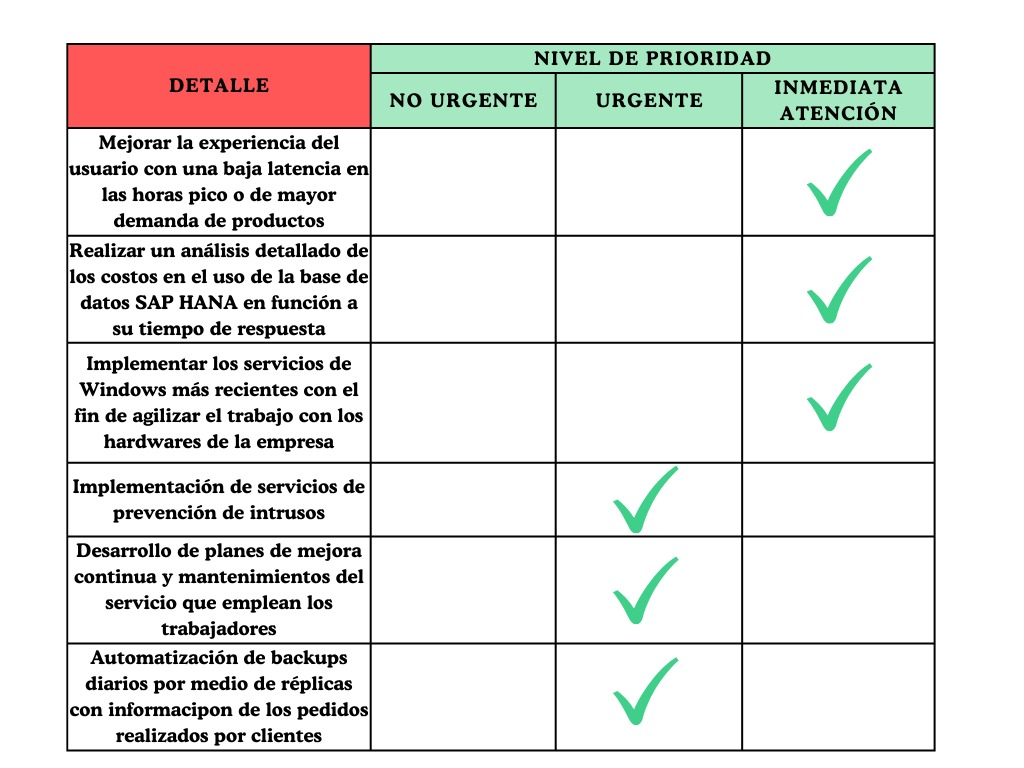
\includegraphics[width=0.9\textwidth]{backlog.jpg}
            \caption{Backlog - requerimientos del negocio}
        \end{figure}
    \newpage
    \subsubsection{Valoración de las capacidades de las TICs}
        \begin{figure}[!ht]
            \centering
            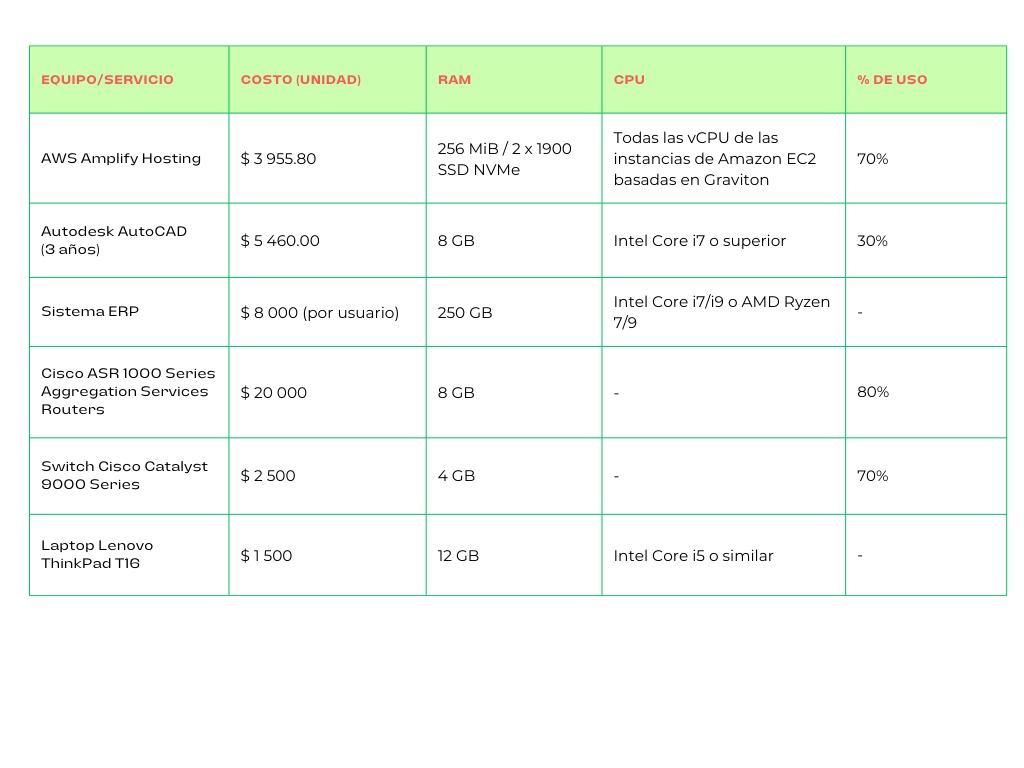
\includegraphics[width=0.8\textwidth]{cuadro_caloracion_capacidades_tic.jpeg}
            \caption{cuadro de la valoración de capacidades de las TIC's de Alicorp}
        \end{figure}

\subsection{Back log de requerimientos del negocio y del área de TI}

    \paragraph*{Automatización de Procesos Comerciales}
        \begin{itemize}
            \item Implementar un sistema que permitan a los clientes corporativos (B2B) realizar pedidos, consultar inventarios, revisar historial de compras y gestionar sus cuentas a través de una plataforma digital. Con ello, se reducirá el tiempo de procesamiento de pedidos, se minimizarán errores humanos, y se mejorará la experiencia del cliente.
            \item Implementar un software que gestione automáticamente la emisión de facturas, envíe recordatorios de pago y procese cobros, integrando todo en el sistema contable. Así se acelerará el ciclo de ventas, se mejorará en la precisión de la facturación y reducción del tiempo de respuesta en la gestión de cuentas por cobrar por el área de Logística.
            \item Desarrollar una experiencia de venta fluida y consistente, ya sea que el cliente interactúe con la marca en tiendas físicas, en línea o a través de aplicaciones móviles. Se verá mejorada la satisfacción del cliente y aumentaran las ventas al ofrecer múltiples canales de compra integrados.
        \end{itemize}
    \paragraph*{Expansión de Mercado}
        \begin{itemize}
            \item Modificar productos existentes para cumplir con las preferencias culturales, regulaciones y condiciones del mercado objetivo. Con ello se aumentarán las probabilidades de éxito al penetrar nuevos mercados ofreciendo productos que se alineen mejor con las expectativas locales.
            \item Colaborar con empresas locales o internacionales para compartir recursos y conocimientos, y entrar más eficientemente en nuevos mercados. Se reducirá el riesgo de entrada en nuevos mercados, habrá mayor acceso a la experiencia local y al capital, y gran potencial para compartir beneficios.
            \item Desarrollar campañas de marketing que se adapten a las peculiaridades de cada mercado, utilizando tanto medios digitales como tradicionales. Mejorando así la efectividad del marketing y el reconocimiento de marca en los mercados nuevos.
        \end{itemize}
    
    \paragraph*{Cumplimiento de Normativas Locales e Internacionales}
        \begin{itemize}
            \item Implementar un sistema de gestión de riesgos para asegurar el cumplimiento de las regulaciones financieras y fiscales tanto a nivel local como internacional.
            \item Realizar auditorías periódicas en la nueva sede para garantizar el cumplimiento de normativas internacionales relacionadas con la seguridad alimentaria, protección de datos y estándares laborales.
            \item Adaptar los procedimientos internos a las normativas locales, asegurando también el cumplimiento de normativas internacionales de comercio y mejores prácticas.
        \end{itemize}

    \paragraph*{Optimización de la Cadena de Suministro}
        \begin{itemize}
            \item Implementar soluciones de automatización en la logística para mejorar la eficiencia en la gestión de inventarios, reducir tiempos de entrega y asegurar el abastecimiento oportuno en la nueva operación.
            \item Integrar herramientas de análisis predictivo que permitan anticipar la demanda del mercado, optimizando el flujo de productos y materiales desde otras sedes.
            \item Fortalecer alianzas estratégicas con proveedores locales y regionales para asegurar la resiliencia de la cadena de suministro .
        \end{itemize}

\subsection{Servicios específicos brindados por proveedores y de manera interna}

\paragraph*{Google Cloud Platform (GCP)}es una plataforma de servicios en la nube que ofrece a las empresas herramientas para computación, almacenamiento, análisis de datos e inteligencia artificial, ayudando a gestionar y escalar sus operaciones tecnológicas de manera eficiente.

\paragraph*{Cisco} Cisco ofrece una amplia gama de servicios y soluciones para empresas, abarcando desde infraestructura de red y seguridad hasta colaboración y gestión de datos. 

\paragraph*{Autodesk} Autodesk ofrece software y servicios diseñados para diseñar, ingeniería y construir y crear contenido digital. Sus soluciones están orientadas a una amplia gama de industrias, incluyendo arquitectura, ingeniería, construcción, manufactura, medios y entretenimiento. 



    \subsubsection{Limitaciones y capacidades de la TI}
    \paragraph*{Capacidades:}
        Cisco proporciona soluciones avanzadas de red que permiten una conectividad segura y eficiente a nivel empresarial, mejorando la comunicación y la transferencia de datos. También ofrece herramientas de ciberseguridad robustas, como firewalls, protección contra amenazas y gestión de políticas de seguridad. Soluciones como Webex facilitan la colaboración remota y la comunicación entre equipos. Proporciona soluciones de almacenamiento y gestión de datos que facilitan la operación y administración de la infraestructura TI.
        Autodesk en un software líder para diseño 3D, CAD, ingeniería y arquitectura, facilitando la creación de modelos detallados y precisos. Sus soluciones son adaptables para diferentes sectores, incluyendo arquitectura, construcción, manufactura y medios digitales. Está constantemente innovando sus productos, integrando tecnologías como inteligencia artificial y realidad aumentada para mejorar la experiencia de usuario.
        Google Cloud crea soluciones escalables para almacenamiento, estadísticas, macrodatos y desarrollo de aplicaciones, permitiendo una adaptación a las necesidades cambiantes del negocio. Proporciona herramientas avanzadas para implementar aprendizaje automático y análisis de datos, apoyando la toma de decisiones basadas en datos. También recursos de capacitación y soporte robusto, ayudando a las empresas a adoptar sus servicios con mayor facilidad y confianza.
    \paragraph*{Limitaciones:}
        Las soluciones de Cisco suelen tener costos elevados de implementación y mantenimiento, lo que puede ser una barrera para empresas con presupuestos limitados. La implementación y gestión de las soluciones puede requerir personal altamente capacitado, aumentando la dependencia de talento especializado. Puede haber limitaciones en la integración con sistemas existentes si no se utilizan estándares compatibles.
        Los costos de licenciamiento pueden ser elevados, especialmente para empresas que requieren múltiples productos o servicios de Autodesk. La complejidad de las herramientas puede requerir una curva de aprendizaje significativa, lo cual implica inversión en capacitación para los empleados. Las aplicaciones suelen requerir hardware potente, lo que puede incrementar los costos de infraestructura TI.
        Google Cloud puede volverse impredecible debido al modelo de precios basado en uso, especialmente en empresas con un consumo elevado de recursos. Requiere una conectividad a Internet estable y rápida, lo cual puede ser un reto en zonas con infraestructura limitada. A pesar de las fuertes medidas de seguridad, algunas industrias pueden tener restricciones legales o reguladoras que dificultan el uso de servicios en la nube.
\subsection{Requerimientos del negocio}
    Desarrollar una plataforma de gestión operativa y administrativa que abarque toda la cadena de valor, desde la producción hasta la distribución, asegurando la calidad en sus productos y precios competitivos en el mercado. 
    Crear y mantener alianzas con proveedores de materias primas, distribuidores y socios tecnológicos para fortalecer la cadena de suministro y mejorar la eficiencia operativa. 
    Fomentar una relación de confianza y lealtad con los clientes a través de programas de fidelización y atención personalizada que aborden sus necesidades de manera rápida y efectiva. 
    Optimizar la logística para garantizar una distribución eficiente y oportuna de los productos en los diferentes canales de venta, minimizando tiempos de entrega y costos operativos. 
    Mantener la seguridad y el buen funcionamiento de los sistemas operativos y la infraestructura tecnológica para asegurar la continuidad del negocio y una experiencia satisfactoria para los clientes. 
    Innovar continuamente en procesos de producción y soluciones tecnológicas para mejorar la competitividad y mantener la rentabilidad del negocio. 
    Asegurar el crecimiento sostenible y la generación de valor para los accionistas mediante una gestión eficiente de los recursos y el desarrollo de productos de alto valor agregado. 
\subsection{Requerimientos de las TICs}
    Implementar soluciones tecnológicas que optimicen la gestión operativa y administrativa, garantizando la calidad y eficiencia en los procesos. 
    Mantener al personal capacitado y al tanto de nuevas tecnologías y actualizaciones en los procedimientos internos y externos. 
    Asegurar que las soluciones tecnológicas estén alineadas con los objetivos estratégicos de Alicorp y las necesidades específicas del sector de consumo masivo. 
    Evaluar e implementar tendencias tecnológicas que mejoren la competitividad de Alicorp, como la automatización en la producción, el uso de big data en la toma de decisiones y la integración de tecnologías IoT en la cadena de suministro. 